\documentclass[tikz,border=5pt]{standalone}
\usepackage{amsmath,amssymb}
\usepackage{tikz}
\usetikzlibrary{calc,arrows.meta}
\begin{document}
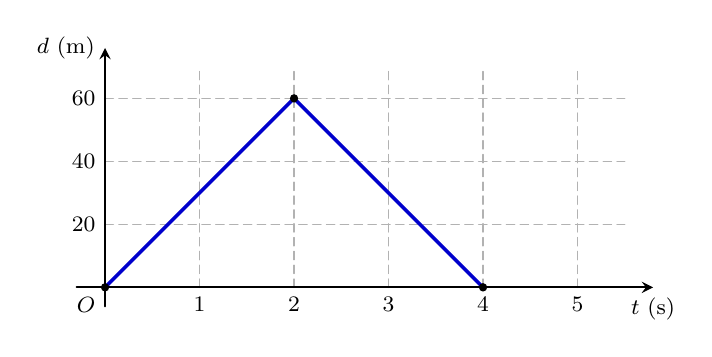
\begin{tikzpicture}[>=stealth, line join=round, line cap=round, font=\footnotesize, xscale=1.2, yscale=0.8]
	% Đường lưới nét đứt
	\foreach \x in {1, 2, 3, 4, 5} {
		\draw[dash pattern=on 3pt off 2pt, gray!60, line width=0.5pt] (\x, 0) -- (\x, 3.5);
	}
	\foreach \y in {1, 2, 3} {
		\draw[dash pattern=on 3pt off 2pt, gray!60, line width=0.5pt] (0, \y) -- (5.5, \y);
	}
	% Trục tọa độ
	\draw[->, thick] (0, -0.3) -- (0, 3.8) node[left] {$d\text{ (m)}$};
	\draw[->, thick] (-0.3, 0) -- (5.8, 0) node[below] {$t\text{ (s)}$};
	% Nhãn trên các trục
	\node[left] at (0, 1) {$20$};
	\node[left] at (0, 2) {$40$};
	\node[left] at (0, 3) {$60$};
	\node[below] at (1, 0) {$1$};
	\node[below] at (2, 0) {$2$};
	\node[below] at (3, 0) {$3$};
	\node[below] at (4, 0) {$4$};
	\node[below] at (5, 0) {$5$};
	\node[below left] at (0, 0) {$O$};
	% Đồ thị chuyển động
	\draw[line width=1.3pt, blue!80!black] (0, 0) -- (2, 3) -- (4, 0);
	\fill[black] (0, 0) circle (1.25pt and 1.9pt);
	\fill[black] (2, 3) circle (1.25pt and 1.9pt);
	\fill[black] (4, 0) circle (1.25pt and 1.9pt);
\end{tikzpicture}
\end{document}
